\documentclass[border=12pt]{standalone}
\usepackage{tikz}
\usepackage{amsmath}
\usetikzlibrary{positioning,arrows.meta,fit,backgrounds,calc}
\begin{document}
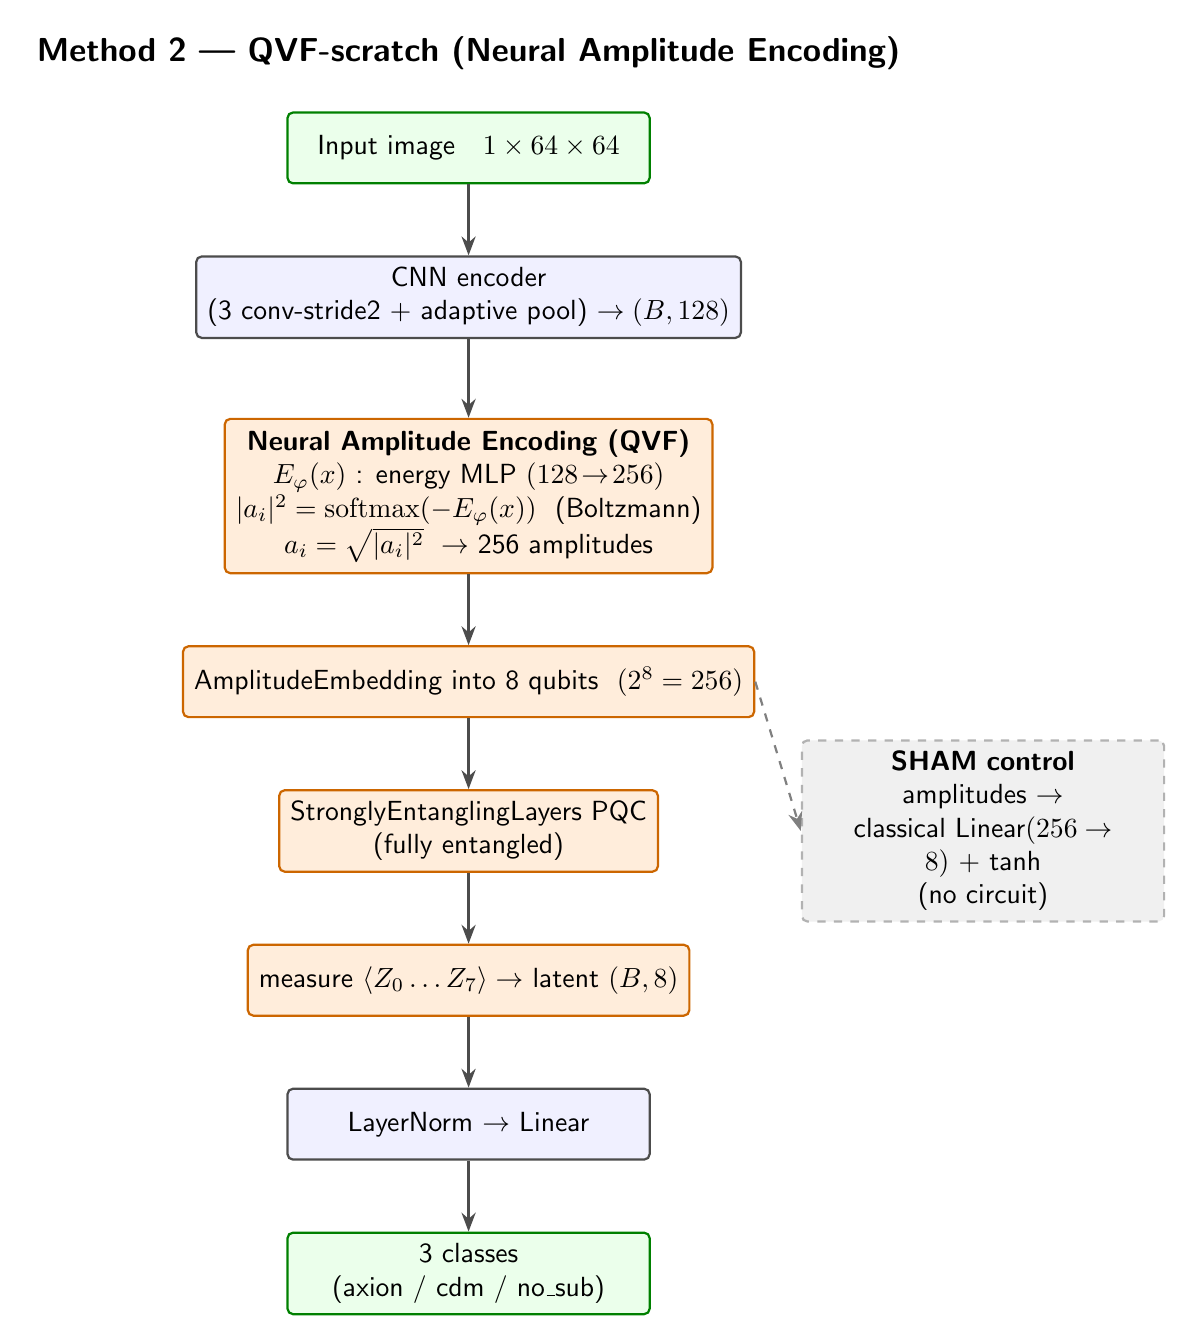
\begin{tikzpicture}[
  font=\sffamily,
  node distance=9mm,
  box/.style={rectangle,rounded corners=2pt,draw=black!70,thick,fill=blue!6,
              minimum height=9mm,minimum width=46mm,align=center,inner sep=4pt},
  qbox/.style={box,fill=orange!14,draw=orange!80!black},
  shbox/.style={box,fill=gray!12,draw=gray!60,dashed},
  io/.style={box,fill=green!8,draw=green!50!black},
  arr/.style={-{Stealth[length=2.4mm]},thick,black!70},
]
\node[io] (img) {Input image\quad$1\times64\times64$};
\node[box,below=of img] (cnn) {CNN encoder\\(3 conv-stride2 + adaptive pool) $\to (B,128)$};
\node[qbox,below=10mm of cnn,minimum width=58mm] (nae)
   {\textbf{Neural Amplitude Encoding (QVF)}\\
    $E_\varphi(x)$ : energy MLP $(128\!\to\!256)$\\
    $|a_i|^2=\mathrm{softmax}(-E_\varphi(x))$ \ (Boltzmann)\\
    $a_i=\sqrt{|a_i|^2}\ \to$ 256 amplitudes};
\node[qbox,below=of nae] (amp) {AmplitudeEmbedding into 8 qubits \ $(2^8=256)$};
\node[qbox,below=of amp] (pqc) {StronglyEntanglingLayers PQC\\(fully entangled)};
\node[qbox,below=of pqc] (z) {measure $\langle Z_0\dots Z_7\rangle \to$ latent $(B,8)$};
\node[box,below=of z] (head) {LayerNorm $\to$ Linear};
\node[io,below=of head] (out) {3 classes\\(axion / cdm / no\_sub)};

\draw[arr] (img)--(cnn);
\draw[arr] (cnn)--(nae);
\draw[arr] (nae)--(amp);
\draw[arr] (amp)--(pqc);
\draw[arr] (pqc)--(z);
\draw[arr] (z)--(head);
\draw[arr] (head)--(out);

\node[shbox,right=18mm of pqc,text width=40mm] (sham)
   {\textbf{SHAM control}\\amplitudes $\to$\\classical Linear$(256\!\to\!8)$ + tanh\\(no circuit)};
\draw[arr,dashed,gray] (amp.east) -- (sham.west);

\node[font=\sffamily\large\bfseries,above=4mm of img]
   {Method 2 — QVF-scratch (Neural Amplitude Encoding)};
\end{tikzpicture}
\end{document}
